\section{Felder}
\textbf{Feldunterscheidung}
\begin{align*}
	 & \vec{E}(x,y,z)                               & \widehat= & \quad\text{statisches Feld}  & \\
	 & \vec{E}(x,y,z,t)                             & \widehat= & \quad\text{quasi-stationäres Feld} & \\
	 & \vec{E}(x,y,z,t)\cdot cos(\omega t -\beta z) & \widehat= & \quad\text{Welle}            &
\end{align*}

\subsection{Elektrostatik}
	Wirbelfreie Felder $\rightarrow$ Gradientenfeld $\rightarrow$ elek. Ladungen
	sind Quellen des $\vec{E}$-Feldes (Skalare Potenzialfkt. $ \varphi $)
	\begin{align*}
		\oprot \vec{E} & = 0 = \oprot \opgrad \varphi & \vec{E} & = -\opgrad \varphi    & \\
		\opdiv \vec{D} & = \rho                 & \vec{D} & = \varepsilon \vec{E} &
	\end{align*}

	\subsubsection{Potential-/Poisson-Gleichung}
		La-Place-Gleichung, wenn $ \rho = 0 $

		\begin{align*}
			\opdiv \opgrad \varphi = \Delta \varphi & = - \dfrac{\rho}{\varepsilon}           \\
			\Delta \varphi + \underbrace{ \dfrac{\opgrad \varepsilon \cdot \opgrad \varphi}{\varepsilon}}_{= 0\texttt{, wenn homogen}}
													& = - \dfrac{\rho (x, y, z)}{\varepsilon}
		\end{align*}

		\textbf{meistens Ziel: Vereinfachung zu 1 Variable}

	\subsubsection{Randwertprobleme, -bedingungen (RB)}
		\textbf{Dirichlet-RB}: Gesuchte Potenzialfunktion $ \varphi $ nimmt an den
		Rändern einen bestimmten Wert an (Bsp.: $\rho_r = 5V$)

		\textbf{Neumann-RB}: Die Normalenableitung $ \tfrac{\partial\varphi}{\partial
				n} $ der Fkt. $ \varphi $ nimmt an den Rändern einen bestimmten Wert an. \\
		(Bsp.: Grenzfläche unterschiedlicher Dielektrika) \\
		\(\frac{\partial \varphi}{\partial n} = \opgrad \varphi \cdot \vec{n}\), \(\vec{n}\): Normalenvektor

	\subsubsection{Green'sche Funktionen}
		\textbullet{\textbf{Skalarpotential} einer Punktladung}
		\[ \varphi (r) = \dfrac{Q}{4 \pi \varepsilon_0 \cdot r} \qquad\left[V\right] \]

		\textbullet{\textbf{E-Feld} einer Punktladung}
		\[ \vec{E}(r) = \dfrac{Q}{4 \pi \varepsilon_0 \cdot r^2}\cdot\vec{e}_r \qquad\left[\frac{V}{m}\right] \]

		\textbullet{\textbf{D-Feld} einer Punktladung}
		\[ \vec{D}(r) = \dfrac{Q}{4 \pi \cdot r^2}\cdot\vec{e}_r \qquad\left[\frac{As}{m^2}=\frac{C}{m^2}\right] \]

		\textbullet{\textbf{Potentialfeld} einer Ladungsdichteverteilung}

		mit $\varphi(\infty)=0$
		\[
			\varphi(x, y, z)=\frac{1}{4 \pi \varepsilon} \iiint_{V^{\prime}}
			\frac{\rho\left(x^{\prime}, y^{\prime},
				z^{\prime}\right)}{\left|\vec{r}-\vec{r}^{\,\prime}\right|} \mathrm{d}
			V^{\prime}
		\]
		wobei:
		\begin{itemize}
			\item \(\vec{r}'\): Ortsvektor zum Punkt der Ladungsmenge
			\item \(\vec{r}\): Ortsvektor zum Aufpunkt \\ (Punkt, an dem das Potential berechnet werden soll)
		\end{itemize}

		mit der Green'schen Funktion $G\left(\vec{r},
			\vec{r}^{\,\prime}\right)=\frac{1}{4 \pi
				\varepsilon\left|\vec{r}-\vec{r}^{\,\prime}\right|}$
		\[ \varphi(x, y, z)=\iiint_{V^{\prime}} G\left(\vec{r}, \vec{r}^{\,\prime}\right) \rho\left(\vec{r}^{\,\prime}\right) \mathrm{d} V^{\prime} \]

		Vereinfachungen bei bekannter Ladungsverteilung:
		\begin{table}[H]
			\centering
			\begin{tabular}{l | c}
				Flächenladungsdichte \(\sigma\) & \(\varphi = \frac{1}{4\pi\epsilon} \iint_A' \frac{\sigma(x',y',z')}{\left|\vec{r} - \vec{r}'\right|} \mathsf{d}A'\) \\
				Linienladungsdichte \(\lambda\) & \(\varphi = \frac{1}{4\pi\epsilon} \int_s' \frac{\lambda(x',y',z')}{\left|\vec{r} - \vec{r}'\right|} \mathsf{d}s'\) \\
				Diskrete Punktladungen & \(\varphi = \frac{1}{4\pi\epsilon} \sum_{i=1}^N \frac{Q_i}{\left|\vec{r} - \vec{r}_i\right|}\)
			\end{tabular}
		\end{table}

	\subsubsection{Elektrischer Dipol}
		{\footnotesize Wird von Prof. Stücke nicht behandelt}
		\\
		Dipolmoment $\vec{p} = Q\cdot\vec{d}$

		\makebox[0pt][l]{
			\begin{minipage}[b]{0.5\columnwidth}
				\input{Figures/Felder/Elektrischer_Dipol_1.tex}
			\end{minipage}
			\begin{minipage}[b]{0.5\columnwidth}
				\input{Figures/Felder/Elektrischer_Dipol_2.tex}
			\end{minipage}
		}

		\makebox[0pt][l]{
			\begin{minipage}[]{0.5\columnwidth}
				\begin{align*}
					\varphi & = \frac{Q}{4\pi\varepsilon_0}\left(\frac{1}{r_1}-\frac{1}{r_2}\right)                                        \\
							& = \frac{Q}{4\pi\varepsilon_0}\cdot\frac{r_2-r_1}{r^2}                                                        \\
					\vec{E} & = -\nabla\varphi                                                                                             \\
							& = \frac{1}{4\pi\varepsilon_0}\cdot\left(\frac{3(\vec{p}\cdot\vec{r})\vec{r}}{r^5}-\frac{\vec{p}}{r^3}\right)
				\end{align*}
			\end{minipage}

			\begin{minipage}[]{0.5\columnwidth}
				\begin{align*}
					\varphi & \approx\frac{Qd\cos\theta}{4\pi\varepsilon_0r^2}                  \\
							& = \frac{1}{4\pi\varepsilon_0}\cdot\frac{\vec{p}\cdot\vec{r}}{r^3}
				\end{align*}
			\end{minipage}
		}

\subsection{Magnetostatik}
	Quellenfreie Wirbelfelder mit \textit{geschlossenen} Feldlinien.

	Keine magnetischen Monopole: $\opdiv \vec{B} = 0$.

	\begin{align*}
		\opdiv \vec{B} &= 0 = \opdiv \oprot \vec{A} & \oprot \vec{H} &= \vec{J} & \vec{B} &= \mu \vec{H} & \\
	\end{align*}

	\subsubsection{Vektorpotential}
		Reine Hilfsgröße, in Analogie zum elek. Skalarpotential $ \varphi $.

		\textbf{Coulomb-Eichung}, wenn $ \opdiv \vec{A} = 0 $, gilt \textbf{nur} für
		zeitunabhängige Felder.
		\begin{align*}
			\Delta \vec{A} & = - \mu \vec{J}  &
			\vec{B}        & = \oprot \vec{A} &
			\left[\vec{A} \right] = \frac{Wb}{m} = \frac{Vs}{m}
		\end{align*}

	\subsubsection{Vektorpotential in Abhängigkeit von der Stromdichte}
		\[
			\vec{A}(x, y, z)=\frac{\mu}{4 \pi} \iiint_{V^{\prime}} \frac{\vec{J}\left(x^{\prime}, y^{\prime}, z^{\prime}\right)}{\left|\vec{r}-\vec{r}^{\,\prime}\right|} d V^{\prime}
		\]

	\subsubsection{Biot-Savart-Gesetz}
		\[
			\vec{H}=\frac{I}{4 \pi} \oint_{C^{\prime}} \opgrad \frac{1}{\left|\vec{r}-\vec{r}^{\,\prime}\right|} \times \mathrm{d} \vec{s}^{\,\prime}
		\]

		mit $\opgrad \frac{1}{\left|\vec{r}-\vec{r}^{\,\prime}\right|}=-\frac{\vec{r}-\vec{r}^{\,\prime}}{\left|\vec{r}-\vec{r}^{\,\prime}\right|^{3}}$

		\[
			\vec{H}=\frac{I}{4 \pi} \oint_{C^{\prime}} \frac{\mathrm{d} \vec{s}^{\,\prime} \times\left(\vec{r}-\vec{r}^{\,\prime}\right)}{\left|\vec{r}-\vec{r}^{\,\prime}\right|^{3}}
		\]

		\begin{itemize}
			\footnotesize
			\item \(\vec{r}'\): Ortsvektor zum Punkt der Ladungsmenge
			\item \(\vec{r}\): Ortsvektor zum Aufpunkt \\ (Punkt, an dem das Magnetfeld berechnet werden soll)
		\end{itemize}

	\subsubsection{Magnetischer Dipol}
		{\footnotesize Wird von Prof. Stücke nicht behandelt}
		\input{Figures/Felder/Magnetischer_Dipol_1.tex}

		Strom $I$ entlang eines Leiters: $\left[\vec{A}\right] = \frac{Vs}{m}$
		\begin{flalign*}
			\vec{A}(r)                      & = \frac{\mu_0 \cdot I}{4 \pi} \int \frac{d \vec{R}}{| \vec{r} - \vec{R}|} = \frac{ \mu_0}{4 \pi} \frac{\vec{m} \times \vec{r}}{r^3} \\
			\vec{B} = \nabla \times \vec{A} & = \frac{\mu_0}{4 \pi} \left(\frac{3(\vec{m} \cdot \vec{r})\vec{r}}{r^5} - \frac{\vec{m}}{r^3}\right)
		\end{flalign*}

\subsection{Quasistationäre Felder (Wechselstrom)}
	Homogenes, Isotropes Medium: $ \varepsilon, \mu, \kappa = \mathtt{kost.} $\\
	Leiter ist quasineutral: $ \rho = 0 $. \(\frac{\partial}{\partial t} \ne 0 \quad \frac{\partial \vec{D}}{\partial t} \ll \vec{J}\)
	\begin{align*}
		\oprot \vec{E} & = -\frac{\partial \vec{B}}{\partial t} = -\mu \frac{\partial \vec{H}}{\partial t} & \opdiv \vec{E} & = 0 & \vec{D} & = \varepsilon\vec{E} & \\
		\oprot \vec{H} & = \vec{J} = \kappa \vec{E}                                                        & \opdiv \vec{B} & = 0 & \vec{B} & = \mu\vec{H}         & \\
		\opdiv \vec{J} & = -\frac{\partial \rho}{\partial t}                                               & \opdiv \vec{H} & = 0 & \vec{J} & = \kappa \vec{E}     &
	\end{align*}

	\subsubsection{Komplexe Feldgrößen}
	\textbullet komplexer Amplitudenvektor / Phasor:
	\begin{equation*}
		\underline{\vec{J}}=\vec{J}\cdot e^{j\varphi}
	\end{equation*}
	\textbullet komplexer Amplituden-Drehzeiger:
	\begin{align*}
		\underline{\vec{J}}(t) & =\underline{\vec{J}} \cdot e ^{j\omega t} = \vec{J} \cdot e^{j(\omega t+\varphi)}
	\end{align*}
	\textbullet Darstellung in karthesischen Koordinaten:
	\begin{align*}
		\underline{\vec{J}} & =\underline{J}_x \cdot \vec{e}_x + \underline{J}_y \cdot \vec{e}_y + \underline{J}_z \cdot \vec{e}_z
	\end{align*}

\subsection{Skineffekt}\label{sec:skineffekt}
	\begin{mdframed}[style=exercise]
		\begin{itemize}
			\item \textbf{Eindringtiefe}/Äquivalente Leitschichtdicke:\\
				\(\boxed{\delta = \frac{1}{\alpha} = \frac{1}{\beta} = \frac{1}{\sqrt{\pi\mu\kappa f}} = \sqrt{\frac{2}{\omega\mu\kappa}}} \quad \left[\delta\right] = m\)
			\item \textbf{Fortpflanzungskonstante: }\\
				\(\underline{\gamma} = \alpha + j \beta = \sqrt{\frac{\omega\mu\kappa}{2}} (1+j) \)
		\end{itemize}
	\end{mdframed}

	\subsubsection{unendlich breiter Leiter}
		\begin{figure}[H]
			\centering
			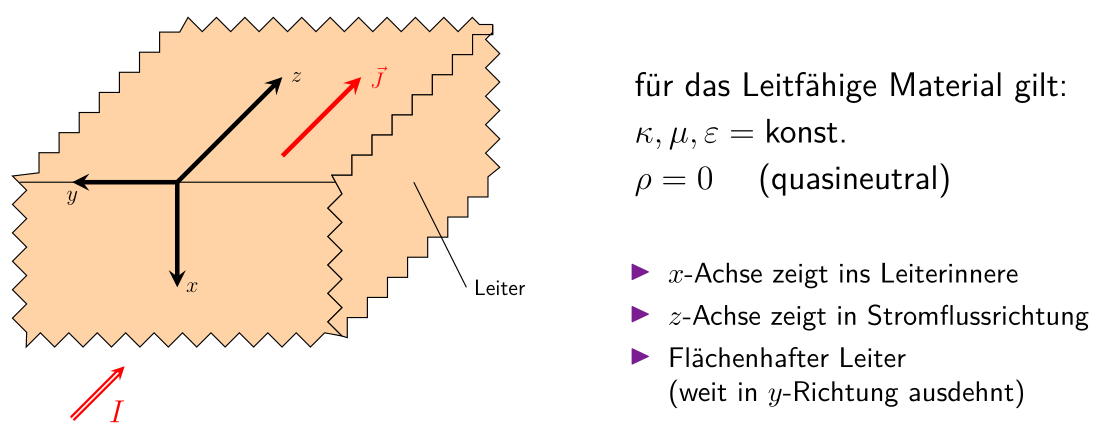
\includegraphics[width=0.9\columnwidth]{Figures/Felder/Skineffekt_unendlichBreit.png}
		\end{figure}
		Lösung durch DGL:
		\begin{align*}
			&\Delta \vec{\underline{E}} - j \omega \mu \kappa \vec{\underline{E}} = 0\\
			&\Delta \vec{\underline{H}} - j \omega \mu \kappa \vec{\underline{H}} = 0
		\end{align*}
		Annahme für Stromdichte:
		\begin{align*}
			\vec{\underline{J}} = \underline{J}_z \cdot \vec{e}_z \quad \text{mit } \vec{\underline{J}} = \kappa \vec{\underline{E}} \quad \vec{\underline{E}} = \underline{E}_z \cdot \vec{e}_z
		\end{align*}
		Lösung des Gleichungssystems ergibt:
		\begin{mdframed}[style=exercise]
			\begin{align*}
				\underline{E}_z(x,t) &= \underline{E}_0 e^{-\underline{\gamma}x} \cdot e^{j \omega t} = \underline{E}_0 e^{-\alpha x} e^{-j \beta x} \cdot e^{j \omega t} \\
				&= E_0 \cdot e^{- \alpha x} \cdot e^{j \left(\omega t - \beta x + \varphi_0\right)}\\
				\underline{H}_y(x,t) &= - \frac{\underline{\gamma}}{j \omega \mu} \underline{E}_z(x,t) = - \sqrt{\frac{\kappa}{\omega \mu}} e^{-j \frac{\pi}{4}} \cdot \underline{E}_z(x,t)\\
				&= - \sqrt{\frac{\kappa}{\omega \mu}} E_0 \cdot e^{- \alpha x} \cdot e^{j \left(\omega t - \beta x + \varphi_0 - \frac{\pi}{4}\right)}\\
			\end{align*}
		\end{mdframed}

	\subsubsection{Rundleiter}
		\input{Figures/Felder/Skineffekt.tex}

		\begin{description}
			\item (Oberflächen)\textbf{widerstand}:
				\begin{flalign*}
					R_{AC} & = \frac{l}{\kappa \cdot A_{\texttt{eff}}} &
					R_{DC} & =\dfrac{l}{\kappa \pi r_0^{2}}              &
					R_F    & = \dfrac{1}{\kappa \delta}                &
				\end{flalign*}

			\item \textbf{Feldstärke} verglichen mit der Oberfläche:\\
				Wenn \(\delta \ll r_0\), kann wie im unendlich breiten Leiter genähert werden mit e-Funktion. 
				Ansonsten keine genaue Aussage möglich (Bessel-Funktion). 

			\item \textbf{Rundleiter - Effektive Fläche}:
				% {\footnotesize
				% 	Gilt nur, wenn kleinste geometrische Abmessung \(> 10\delta\)
				% }
				\begin{align*}
					A_{\texttt{eff}} & = A_{\texttt{ges}} - A_{\sigma} = r_0^2\pi-(r_0-\delta)^2\pi = 2\cdot \pi \delta \left( r_0-\dfrac{\delta }{2}\right)
				\end{align*}
		\end{description}

	\subsubsection{Näherungen für Skineffekt im Rundleiter}
		\begin{figure}[H]
			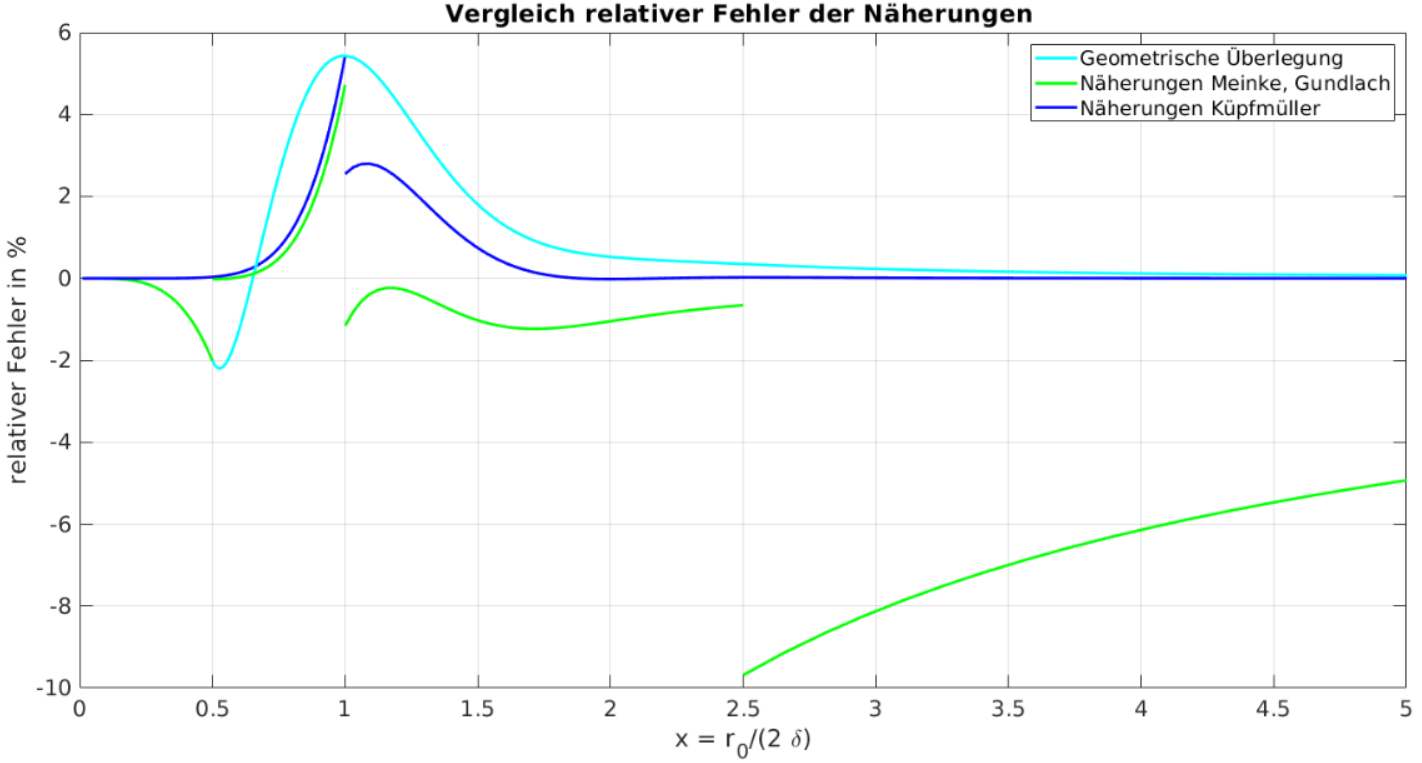
\includegraphics[width=0.98\columnwidth]{Figures/Felder/Skineffekt_Vergleich.png}
		\end{figure}
		\begin{description}
			\item \textbf{Geometrische} Beschreibung (Fehler $ < 6\% $)
				\begin{align*}
					\frac{R_{AC}}{R_{DC}} & =
					\begin{dcases}
						1                                                & \text{für} \quad r_0 < \delta    \\
						\frac{r_0^2}{2\cdot \delta \cdot r_0 - \delta^2} & \text{für} \quad r_0 \geq \delta
					\end{dcases}
				\end{align*}

			\item \textbf{Bessel}-Funktion (Fehler $ < 6 \% $) [Küpfmüller]:
				\begin{align*}
					\frac{R_{AC}}{R_{DC}} & =
					\begin{dcases}
						1 + \frac{1}{3}x^4              & \text{für} \qquad x < 1 \\
						x + \frac{1}{4} + \frac{3}{64x} & \text{für} \qquad x > 1 \\
					\end{dcases} \\
					\frac{X_{AC}}{R_{DC}} & =
					\begin{dcases}
						x^2\left( 1-\frac{x^4}{6} \right)   & \text{für} \qquad x < 1 \\
						x- \frac{3}{64x} + \frac{3}{128x^2} & \text{für} \qquad x > 1 \\
					\end{dcases}
				\end{align*}
				\[
					\boxed{x=\frac{r_0}{2\delta}} \qquad r_0 \, \hat{=} \textnormal{ Außenradius} \qquad X_{AC} = \omega L_i
				\]

			\item \textbf{Empirische} Beschreibung (Fehler $ < 10\% $) [Meinke, Gundlach]:
				\begin{align*}
					\frac{R_{AC}}{R_{DC}} & =
					\begin{dcases}
						1                                                & \text{für} \quad r_0 < \delta                      \\
						1+ \left( \frac{r_0}{2,65\cdot \delta} \right)^4 & \text{für} \quad \delta < r_0 < 2\delta            \\
						\frac{r_0}{2 \cdot\delta} + \frac{1}{4}          & \text{für} \quad 2\delta < r_0 < 5\delta \quad (1) \\
						\frac{r_0}{2\cdot \delta}                        & \text{für} \quad 5\delta < r_0 \quad (2)
					\end{dcases}
				\end{align*}
				\footnotesize Anmerkung: (1) $\widehat{=}$ Kreisring mit Näherung \quad
				(2) $\widehat{=}$ Ring mittig
		\end{description}

\subsection{E-Felder an Grenzflächen}
	\subsubsection{Dielektrische Grenzfläche}
		\textbf{Querschichtung}:
		\begin{align*}
			D_{1n} & = D_{2n} & \varepsilon_1 E_{1n} & =\varepsilon_2 E_{2n} &
		\end{align*}
		Schwächeres E-Feld bei höherem $ \varepsilon $.

		\vspace{0.5em}
		\textbf{Längsschichtung}:
		\begin{align*}
			E_{1t} & = E_{2t} & \frac{D_{1t}}{\varepsilon_1} & = \frac{D_{2t}}{\varepsilon_2} &
		\end{align*}

		Höheres D-Feld (mehr Ladungen) bei höherem $ \varepsilon $.

		\vspace{0.5em}
		\textbf{Schrägschichtung}:
		\begin{align*}
			& \frac{\tan( \alpha_1)}{\tan( \alpha_2)} = \frac{E_{1t}/E_{1n}}{E_{2t}/E_{2n}} = \frac{D_{2n}/\varepsilon_2}{D_{1n}/\varepsilon_1} = \frac{ \varepsilon_1}{\varepsilon_2}
		\end{align*}

	\subsubsection{Grenzfläche Dielektrikum-Leiter}
		Ladungen verschieben sich so lange, bis im Leiter kein Feld mehr herrscht.
		$\rightarrow E_{2t}, E_{2n}, D_{2t}, D_{2n} = 0 $

		\vspace{0.5em}
		\textbf{Längsschichtung}:
		\begin{align*}
			E_{1t} & = E_{2t} = 0 & D_{1t} & =\varepsilon_1 E_{1t} = 0 &
		\end{align*}
		Felder stehen stets senkrecht auf elek. Leitern.

		\vspace{0.5em}
		\textbf{Querschichtung}:
		\begin{align*}
			D_{1n} - D_{2n} & = \frac{Q}{A} & D_{1n} & = \frac{Q}{A} & E_{1n} & = \frac{Q}{\varepsilon_1 A} &
		\end{align*}

		D-Feld entspricht der Flächenladungsdichte des Leiters.

	\subsubsection{Grenzfläche an magn. Feldern}
		\textbf{Querschichtung}:
		\begin{align*}
			B_{1n} & = B_{2n} & \mu_1 H_{1n} & =\mu_2 H_{2n} &
		\end{align*}
		Schwächeres H-Feld bei höherem $ \mu $.\\

		\textbf{Längsschichtung}:
		\begin{align*}
			H_{1t} & = H_{2t} & \frac{B_{1t}}{\mu_1} & = \frac{B_{2t}}{\mu_2} &
		\end{align*}

		Höheres B-Feld (mehr Fluss) bei höherem $ \mu $.

		\vspace{0.5em}
		\textbf{Schrägschichtung}:
		\begin{align*}
			& \frac{\tan( \alpha_1)}{\tan( \alpha_2)} = \frac{ \mu_1}{\mu_2}
		\end{align*}
